%
% Complete documentation on the extended LaTeX markup used for Insight
% documentation is available in ``Documenting Insight'', which is part
% of the standard documentation for Insight.  It may be found online
% at:
%
%     http://www.itk.org/

\documentclass{InsightArticle}

\usepackage[dvips]{graphicx}
\usepackage{subfigure}

%%%%%%%%%%%%%%%%%%%%%%%%%%%%%%%%%%%%%%%%%%%%%%%%%%%%%%%%%%%%%%%%%%
%
%  hyperref should be the last package to be loaded.
%
%%%%%%%%%%%%%%%%%%%%%%%%%%%%%%%%%%%%%%%%%%%%%%%%%%%%%%%%%%%%%%%%%%
\usepackage[dvips,
	bookmarks,
	bookmarksopen,
	backref,
	colorlinks,linkcolor={blue},citecolor={blue},urlcolor={blue},
]{hyperref}


%  This is a template for Papers to the Insight Journal.
%  It is comparable to a technical report format.

% The title should be descriptive enough for people to be able to find
% the relevant document.
\title{Conformal Flattening ITK Filter}

% Increment the release number whenever significant changes are made.
% The author and/or editor can define 'significant' however they like.
\release{0.00}

% At minimum, give your name and an email address.  You can include a
% snail-mail address if you like.
\author{Yi Gao$^{1}$, John Melonakos$^{1}$, and Allen Tannenbaum$^{1}$}
\authoraddress{$^{1}$Georgia Institute of Technology, Atlanta, GA\\
}

\begin{document}

	\newif\ifpdf
	\ifx\pdfoutput\undefined
  \pdffalse
	\else
  \pdfoutput=1
  \pdftrue
	\fi


	\ifpdf
	\else
  %
  % Commands for including Graphics when using latex
  %
  \DeclareGraphicsExtensions{.eps,.jpg,.gif,.tiff,.bmp,.png}
  \DeclareGraphicsRule{.jpg}{eps}{.jpg.bb}{`convert #1 eps:-}
  \DeclareGraphicsRule{.gif}{eps}{.gif.bb}{`convert #1 eps:-}
  \DeclareGraphicsRule{.tiff}{eps}{.tiff.bb}{`convert #1 eps:-}
  \DeclareGraphicsRule{.bmp}{eps}{.bmp.bb}{`convert #1 eps:-}
  \DeclareGraphicsRule{.png}{eps}{.png.bb}{`convert #1 eps:-}
	\fi


	\maketitle


	\ifhtml
	\chapter*{Front Matter\label{front}}
	\fi


	% The abstract should be a paragraph or two long, and describe the
	% scope of the document.
	\begin{abstract}
		\noindent This paper describes the Insight Toolkit (ITK) Conformal
		Flattening filter: itkConformalFlatteningFilter. This ITK filter
		is an implementation of a paper by Sigurd Angenent, et al., ``On
		the Laplace-Beltrami Operator and Brain Surface Flattening''
		\cite{angenent1999lbo}. This filter performs an angle preserving
		map of any genus zero (i.e. no handles) surface to the sphere or,
		alternatively, to the plane. In this paper, we describe our code
		and provide the user with enough details to reproduce the results
		which we present in this paper. This filter has a variety of
		applications including the flattening of brain surfaces, which was
		the initial motivation for this work.
	\end{abstract}

	\tableofcontents

	The folding and wrapping of brain surfaces presents researchers with
	difficulties in obtaining a more intuition-based surface
	rendering. In recent years, a number of methods have been proposed
	to map the brain surface to a plane or a sphere. Most of the
	previous methods are derived to preserve local area or length. Like
	in the work of \cite{davatzikos1996} and \cite{macDonald1994}, a
	parameterized deformable surface whose topology is mappable to a
	sphere is fitted. Thus the brain surface can be represented on a
	planar map using spherical coordinates. Also, as in
	\cite{carman1995} and \cite{schwartz1989}, quasi-isometrics and
	quasi-conformal flattening schemes are used to flatten the brain
	surface. Those methods are more functional minimizing schemes and
	hence bijectivity can not be guaranteed.  In the paper
	\cite{angenent1999lbo}, an bijective angle preserving conformal
	flattening scheme is proposed. See the end of
	section~\ref{sec:brain-flat} for a definition of angle preserving.

	The algorithm obtains the explicit form of the flattening map by
	solving a partial differential equation on the surface using the
	finite element method (FEM). The mapping is a bijection thus the
	triangles do not flip and the original structure can be restored by
	inverse mapping.

	\section{Algorithm Details}

	\subsection{Mathematical manipulation}
  Denote the genus zero surface which is to be flattened as $\Sigma$.
  $\Sigma$ can be mapped to a plane using the algorithm proposed in
  \cite{angenent1999lbo}. The mapping is conformal thus the angles are
  preserved. Furthermore, the plane can be mapped to a sphere, using
  standard stereographic projection.
  
  It is proven in the appendix of \cite{angenent1999lbo} that the mapping
  $z$, defined on $\Sigma$, satisfying is the following:
  \begin{eqnarray}
    \triangle z = (\frac{\partial}{\partial u} - i\frac{\partial}{\partial v})\delta_p 
    \label{pde}
  \end{eqnarray}
  
  where $p$ is an (arbitrary) point on $\Sigma$. The funtion $z$ maps
  $\Sigma \backslash \{p\}$ to the complex plane $\mathbf{C}$. Then by
  standard sterographic projection, the complex plane is mapped to a
  sphere excluding only the north pole.

  \subsection{Numerical scheme}
  The mapping $z$ is defined on the surface. In the numerical
  manipulation where the surface is denoted as a triangulated mesh,
  solving of the equation (\ref{pde}) is carried out by FEM.
  
  In the discrete configuration, $z$ is approximated by a piecewise
  linear function on the triangulated mesh. Denote the
  finite-dimensional space $PL(\Sigma)$ of piecewise linear functions
  on $\Sigma$. To solve equation (\ref{pde}), first its right side
  should be approximated. For any function $f$ smooth in a
  neighborhood of $p$,
  \begin{eqnarray}
    && \int\int_{\Sigma} f (\frac{\partial}{\partial u} - i\frac{\partial}{\partial v})\delta_p \mathrm{d}S \nonumber \\
    &=& - \int\int_{\Sigma}(\frac{\partial}{\partial u} - i\frac{\partial}{\partial v})f \delta_p(w) \mathrm{d}S \nonumber \\
    &=& -(\frac{\partial f}{\partial u} - i\frac{\partial f}{\partial v})\delta_p \label{rightSideOfPDE}
  \end{eqnarray}  
  Thus $\forall f \in PL(\Sigma)$, given that the point $p$ lies in
  the cell composed by three points $A$, $B$, and $C$, the quantity of
  (\ref{rightSideOfPDE}) is determined by the values of $f$ on $A$,
  $B$, and $C$.
  
  On the triangle $\triangle ABC$, choose the $u$ and $v$ axes such
  that $A$ and $B$ are along $u$ axis and the positive direction of
  axis $v$ is pointing to the point $C$. So,
  \begin{eqnarray}    
    \frac{\partial f}{\partial u} &=& \frac{f_B - f_A}{||B - A||} \nonumber \\
    \frac{\partial f}{\partial v} &=& \frac{f_C - f_E}{||C - E||} \nonumber
  \end{eqnarray}  
  in which E is the orthogonal projection of $C$ on $AB$ and can be
  computed by:
  \begin{eqnarray}  
    E = A + \theta(B-A) \nonumber
  \end{eqnarray}  
  where
  \begin{eqnarray}  
    \theta = \frac{<C-A, B-A>}{||B-A||^2} \nonumber
  \end{eqnarray}  
  in which $<,>$ denotes inner product.
  
  Thus $\forall f \in PL(\Sigma)$, 
  \begin{eqnarray}  
    (\frac{\partial f}{\partial u} - i\frac{\partial f}{\partial v})\delta_p = 
    \frac{f_A - f_B}{|| B - A ||} + i\frac{f_c-(f_A + \theta(f_B - f_A))}{||C - E||} \label{Rinteqn}
  \end{eqnarray}  
  
  Next we are going to perform the finite element solution of the
  mapping in the function space $PL(\Sigma)$.
  
  FEM theory indicates that the solver function $z=x+iy$ for equation
  (\ref{pde}) is the minimizer of the Dirichlet functional:
  \begin{eqnarray}  
    \mathbf{D}(z):=\frac{1}{2}\int\int_{\Sigma}[ |\nabla z|^2 + 2z (\frac{\partial}{\partial u} - i\frac{\partial}{\partial v})\delta_p ]\mathrm{d}S \label{DirichletFunctional}
  \end{eqnarray}      
  $z$ satisfies equation(\ref{pde}) if and only if $\forall$ smooth
  function $f$,
  \begin{eqnarray}  
    \int\int_{\Sigma} \nabla z \cdot \nabla f \mathrm{d}S = (\frac{\partial f}{\partial u} - i\frac{\partial f}{\partial v})|_p \label{FEM}
  \end{eqnarray}    
  To find the function in $PL(\Sigma)$ satisfying equation(\ref{FEM}),
  we define a set of basis $\phi_P$ in the $PL(\Sigma)$ as,
  \begin{eqnarray}  
    \phi_P(P) &=& 1 \nonumber \\
    \phi_P(Q) &=& 0, \forall Q \ne P \nonumber \\
    \phi_P(P) && is \quad linear \quad on \quad each \quad triangle \label{basis}
  \end{eqnarray}  
  Then function $z$ can be expressed as a linear combination of the
  basis:
  \begin{eqnarray}  
    z = \sum_{P:\quad vertex \quad of \quad \Sigma} z_P \phi_P \label{zInBasis}
  \end{eqnarray}  
  By this we convert the original problem into solving for the complex
  vector $\vec{z}=(z_P)$:
  \begin{eqnarray}  
    \sum_P z_P \int\int \nabla \phi_P \cdot \nabla \phi_Q \mathrm{d}S = \frac{\partial \phi_Q}{\partial u}(p) - i \frac{\partial \phi_Q}{\partial v}(p)
    \label{allQ}
  \end{eqnarray}  
  Denote matrix $D_{PQ}$ as
  \begin{eqnarray}  
    D_{PQ} = \int\int \nabla \phi_P \cdot \nabla \phi_Q \mathrm{d}S  \label{Dpq}
  \end{eqnarray}  
  The off-diagonal elements of $D$ can be computed by:
  \begin{eqnarray}  
    \{ \mathbf{D} \}_{P,Q } = -\frac{1}{2}(ctg\angle R + ctg\angle S), \quad P \ne Q  \label{ctg}
  \end{eqnarray}  
  \begin{figure}
		\begin{center}
			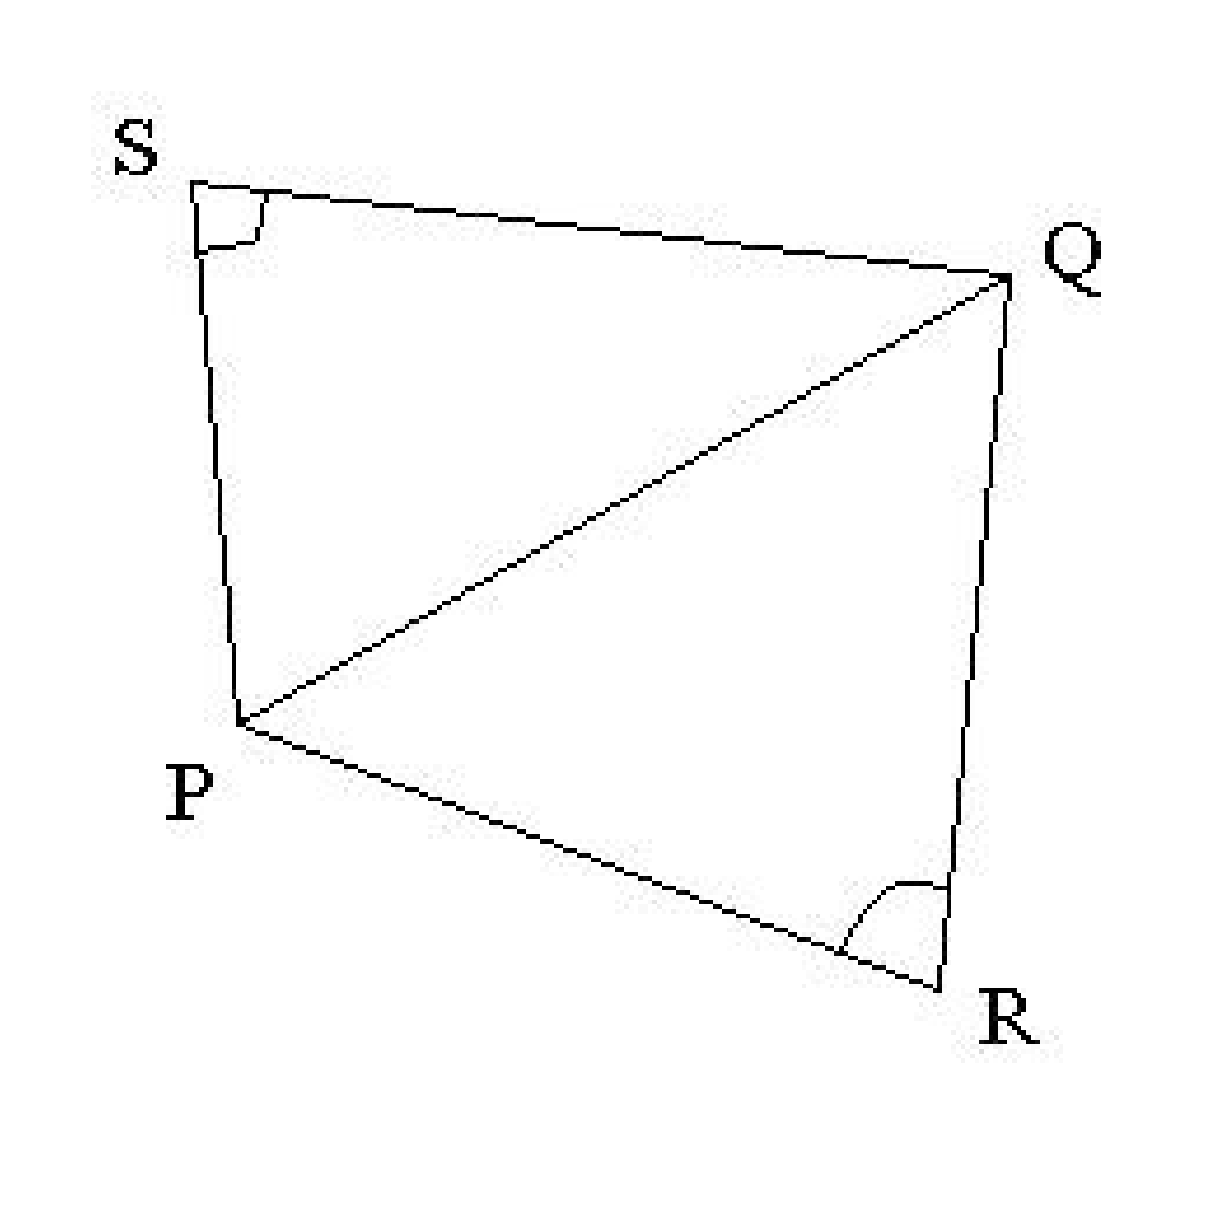
\includegraphics[width=7cm]{PntPQRS.eps} \caption{Triangle} \label{PntPQRS}
    \end{center}
  \end{figure}  
  The points are illustrated in figure (\ref{PntPQRS}).  
  
  Also, since
  \begin{eqnarray}  
    \sum_P D_PQ = \sum_P \int \nabla \phi_P \cdot \nabla \phi_Q = \int \nabla 1 \cdot \nabla \phi_Q = 0
  \end{eqnarray}
  Thus the diagonal elements of matrix D can be obtained by:
  \begin{eqnarray}
    \mathbf{D}_{PP} = -\sum_{P \ne Q}D_PQ \label{diagonalOfD}
  \end{eqnarray}    
  Write each $z_p$ as $z_p=x_p + iy_p$, then
  equation (\ref{allQ}) can be written separately as:
  \begin{eqnarray}
    \sum_{P}x_p D_{PQ} &=& \frac{\partial \Phi(Q)}{\partial u}(P) \nonumber\\
    \sum_{Q}y_p D_{PQ} &=& -\frac{\partial \Phi(Q)}{\partial v} (P)
  \end{eqnarray}  
  denote:
  \begin{eqnarray}
    \vec{a} = (a_Q) &=& \frac{\partial \Phi(Q)}{\partial u}(P) \nonumber \\
    \vec{b} = (b_Q) &=& -\frac{\partial \Phi(Q)}{\partial v} (P)
  \end{eqnarray}  
  so we have:
  \begin{eqnarray}
    \mathbf{D}\vec{x} &=& \vec{a} \nonumber \\
    \mathbf{D}\vec{y} &=& \vec{b} \label{z}
  \end{eqnarray}    
  $\forall \quad point \quad Q$:
  \begin{eqnarray}
    a_Q - ib_Q := \left\{
    \begin{array}{lcl}
      0 & for & Q \notin {A, B, C} \\
      \frac{-1}{||B-A||} + i\frac{1-\theta}{||C-E||} & for & Q = A \\
      \frac{1}{||B-A||} + i\frac{\theta}{||C-E||} & for & Q = B \\
      i\frac{-1}{||C-E||} & for & Q = C
    \end{array} \right. \label{ab}
  \end{eqnarray}      
	With vectors $a$, $b$, and matrix $D$, we can solve the linear
	equation to obtain the mapping. The matrix $D$ is sparce, symmetric
	and positively defined, hence is suitable to being solved by the
	conjugate gradient method.

	\section{User's Guide}

	The conformal flattening filter takes an ITK mesh as input and will
	generate another ITK mesh as output. The usage is basically the same
	as other mesh to mesh filters in ITK.

	\subsection{Basic usage}
	The filter is instaintiated by:
	\begin{verbatim}
		typedef itk::ConformalFlatteningFilter< MeshType, MeshType>  FilterType;
		FilterType::Pointer filter = FilterType::New();
	\end{verbatim}
	Then the input can be set and results can be obtained by:
	\begin{verbatim}
		filter->SetInput( mesh ); 
	\end{verbatim}
	and
	\begin{verbatim}
		newMesh = filter->GetOutput(); 
	\end{verbatim}

	\subsection{More about APIs}
	The filter has several APIs for further manipulation of the output.
	
	\begin{enumerate}
	\item setPointP function. On the right side of equation (\ref{pde}),
	the $\delta_p$ function depands on the location of the point
	\emph{p}. Basically, this point will be mapped to infinity on the
	plane and the north-pole of the sphere. Hence the selection of the
	point \emph{p} determines which patch on the original mesh is mapped
	up to the north pole.

	The API setPointP takes an integer as input indicating the cell
	number in which the point \emph{p} lies. It's a good choice to set
	the point \emph{p} where the local surface is relatively flat, i.e.,
	having a small local curvature. However the computation of curvature
	can be done by the vtkCurvatures filter. In order to make this
	filter independent of VTK, this feature is not included in the
	filter and is left to the user. If setting the point \emph{p} at
	some flat area is crucial, we suggest that user first use
	vtkCurvatures to obtain the number of cells having low curvatures
	and then call this function using one of the cells with a low
	curvature.

	\item The switch functions mapToPlane and mapToSphere determine the
	output to be either a plane or a sphere, the sphere being the
	default. The difference between the two mappings is simply a
	stereographic projection from the plane to the sphere. Simply by
	\begin{verbatim}
		filter->mapToSphere( ); 
	\end{verbatim}
	or
	\begin{verbatim}
		filter->mapToPlane( ); 
	\end{verbatim}
	users can switch between two different outputs.
	
	\item setScale function. The mapping, calculated from the equation
	(\ref{pde}), is dependent on the number of the nodes within the
	mesh. Given a mesh of a large number of nodes and cells, the image
	of the flattening mapping, is constrained in a small range around
	origin. To make it cover a sufficient area of the plane and further
	get a reasonable result from stereographic projection, re-scale of
	the flattened plane is needed. This function is used to set the
	scale factor, by:
	\begin{verbatim}
		filter->setScale( scale factor ); 
	\end{verbatim}
	For a mesh of around several thousands of nodes, a factor of 100 is likely to get a 
	good result. The factor should grow as the number of nodes grows.	
	\end{enumerate}

	\section{The Filter Test}
  Here we explain how the reader may reproduce our results. This
  section contains details about the test we include with the
  submission of this ITK filter. We have provided $nice.vtk$ which is
  a synthetic genus zero mesh. We set this as the first parameter to
  the itkConformalFlatteningFilterTest and we set the output filename
  for the flattend mesh as the second parameter, as follows:

	\begin{verbatim}
		> ./itkConformalFlatteningFilterTest nice.vtk niceFlat.vtk
	\end{verbatim}

  \noindent In Figure~\ref{fig:original}, we show the original
  $nice.vtk$ data, which is colored according to mean curvature. In
  Figure~\ref{fig:nice}, we show the surface view and in
  Figure~\ref{fig:nice-mesh}, we show the triangulated mesh.

  \begin{figure}[t]
		\begin{center}
			\subfigure[Original Surface]{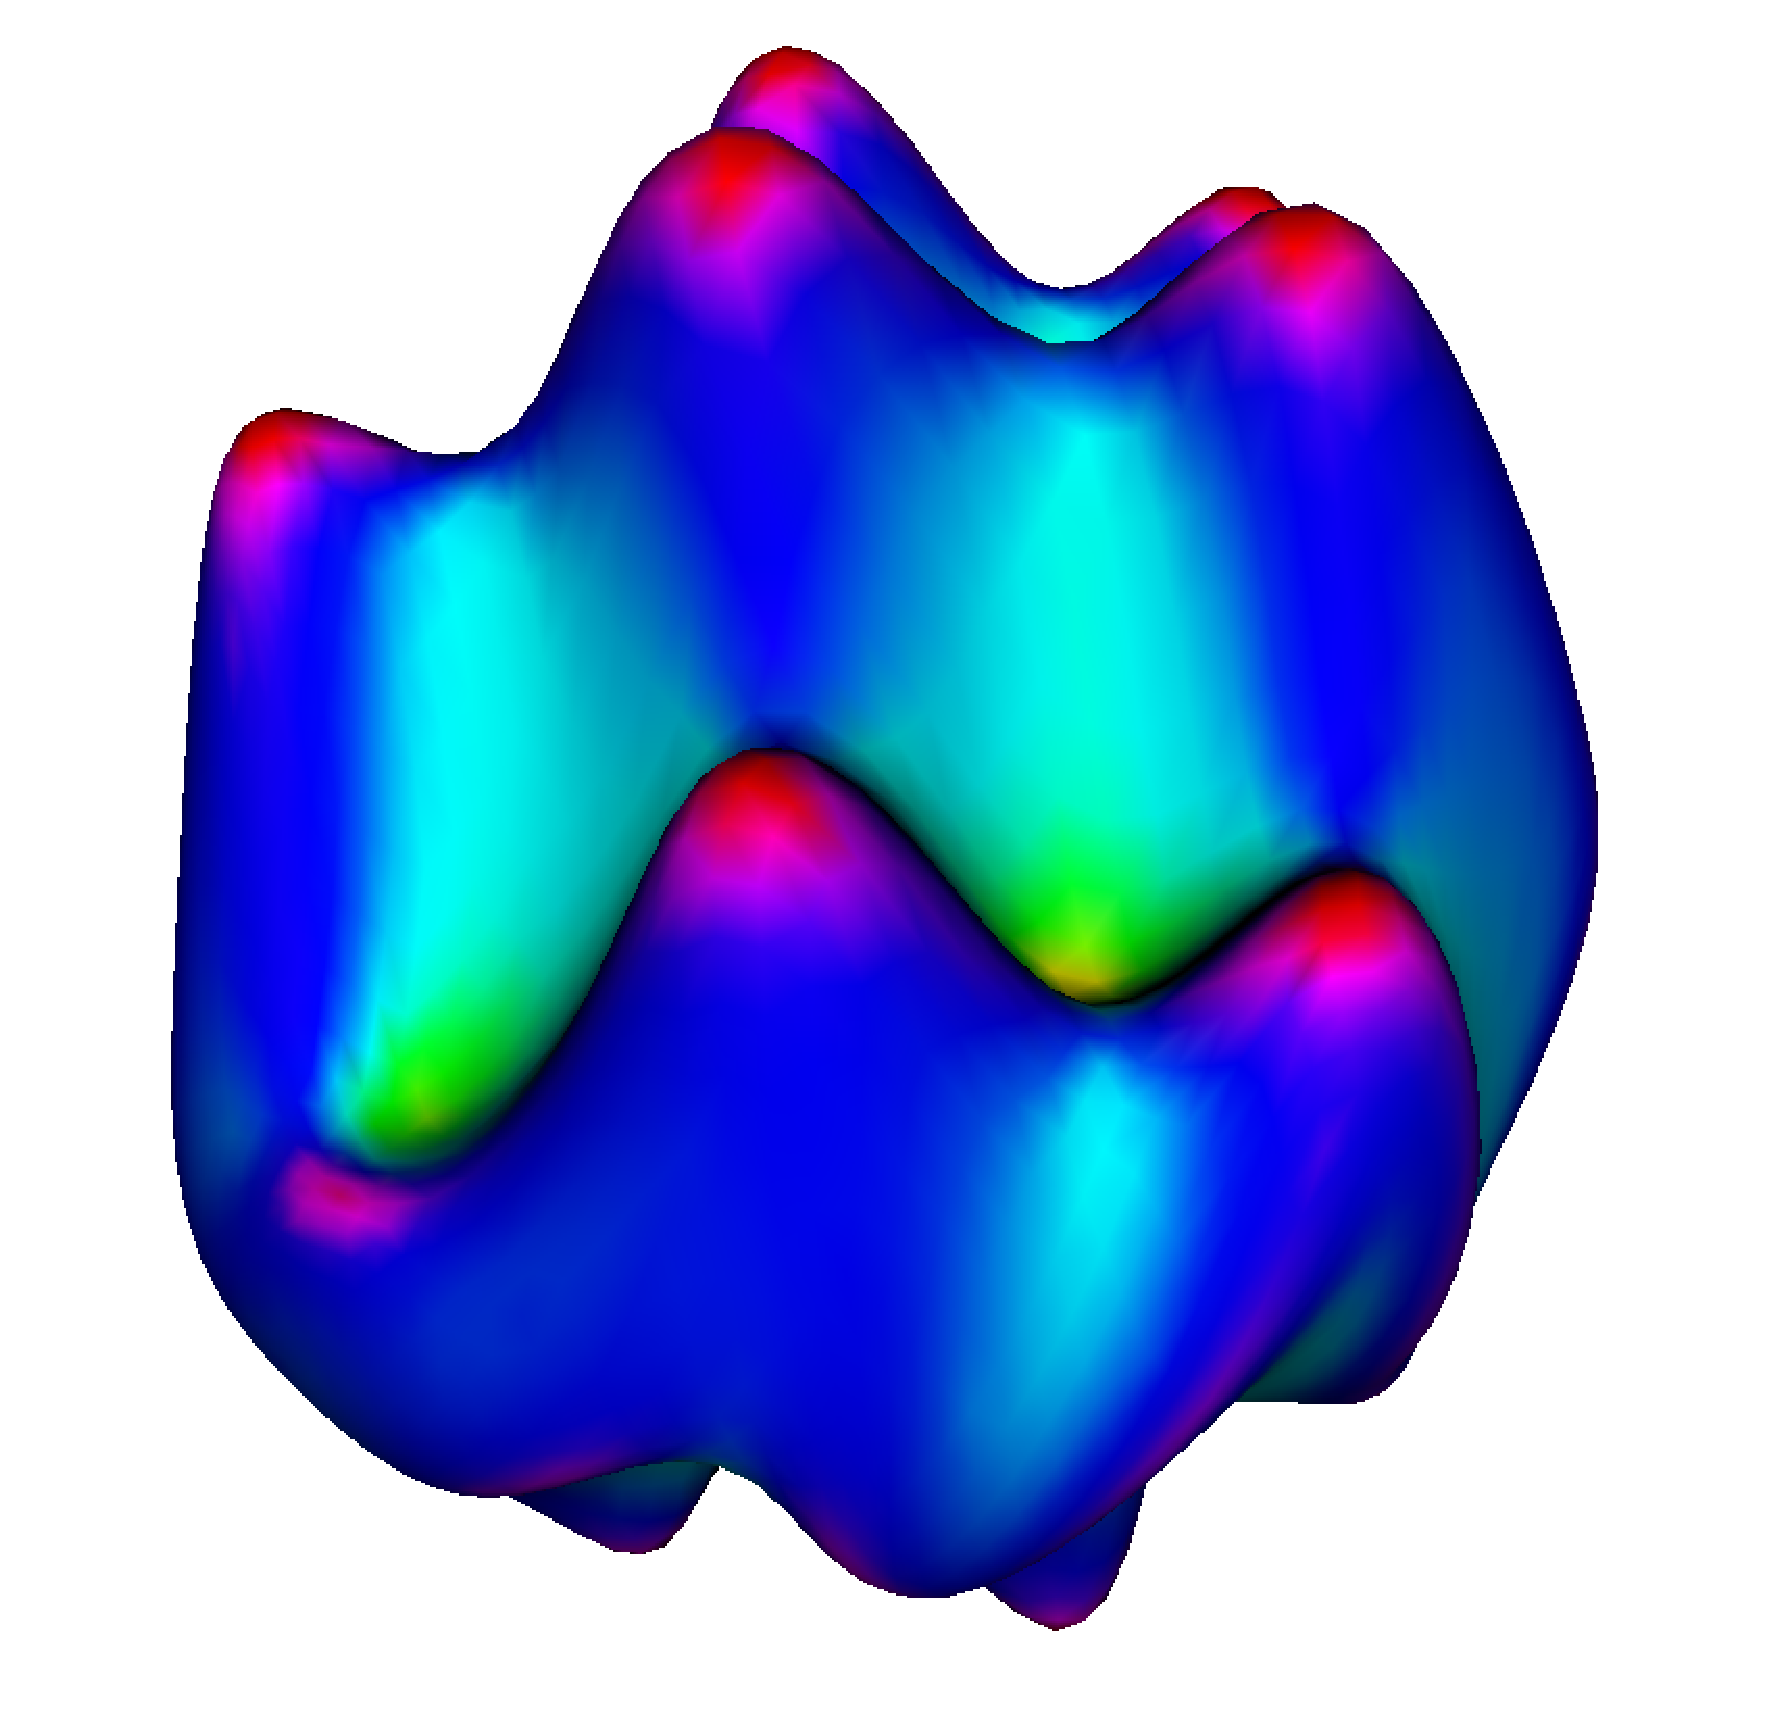
\includegraphics[width=5cm]{nice.eps} \label{fig:nice}}
			\subfigure[Original Mesh]{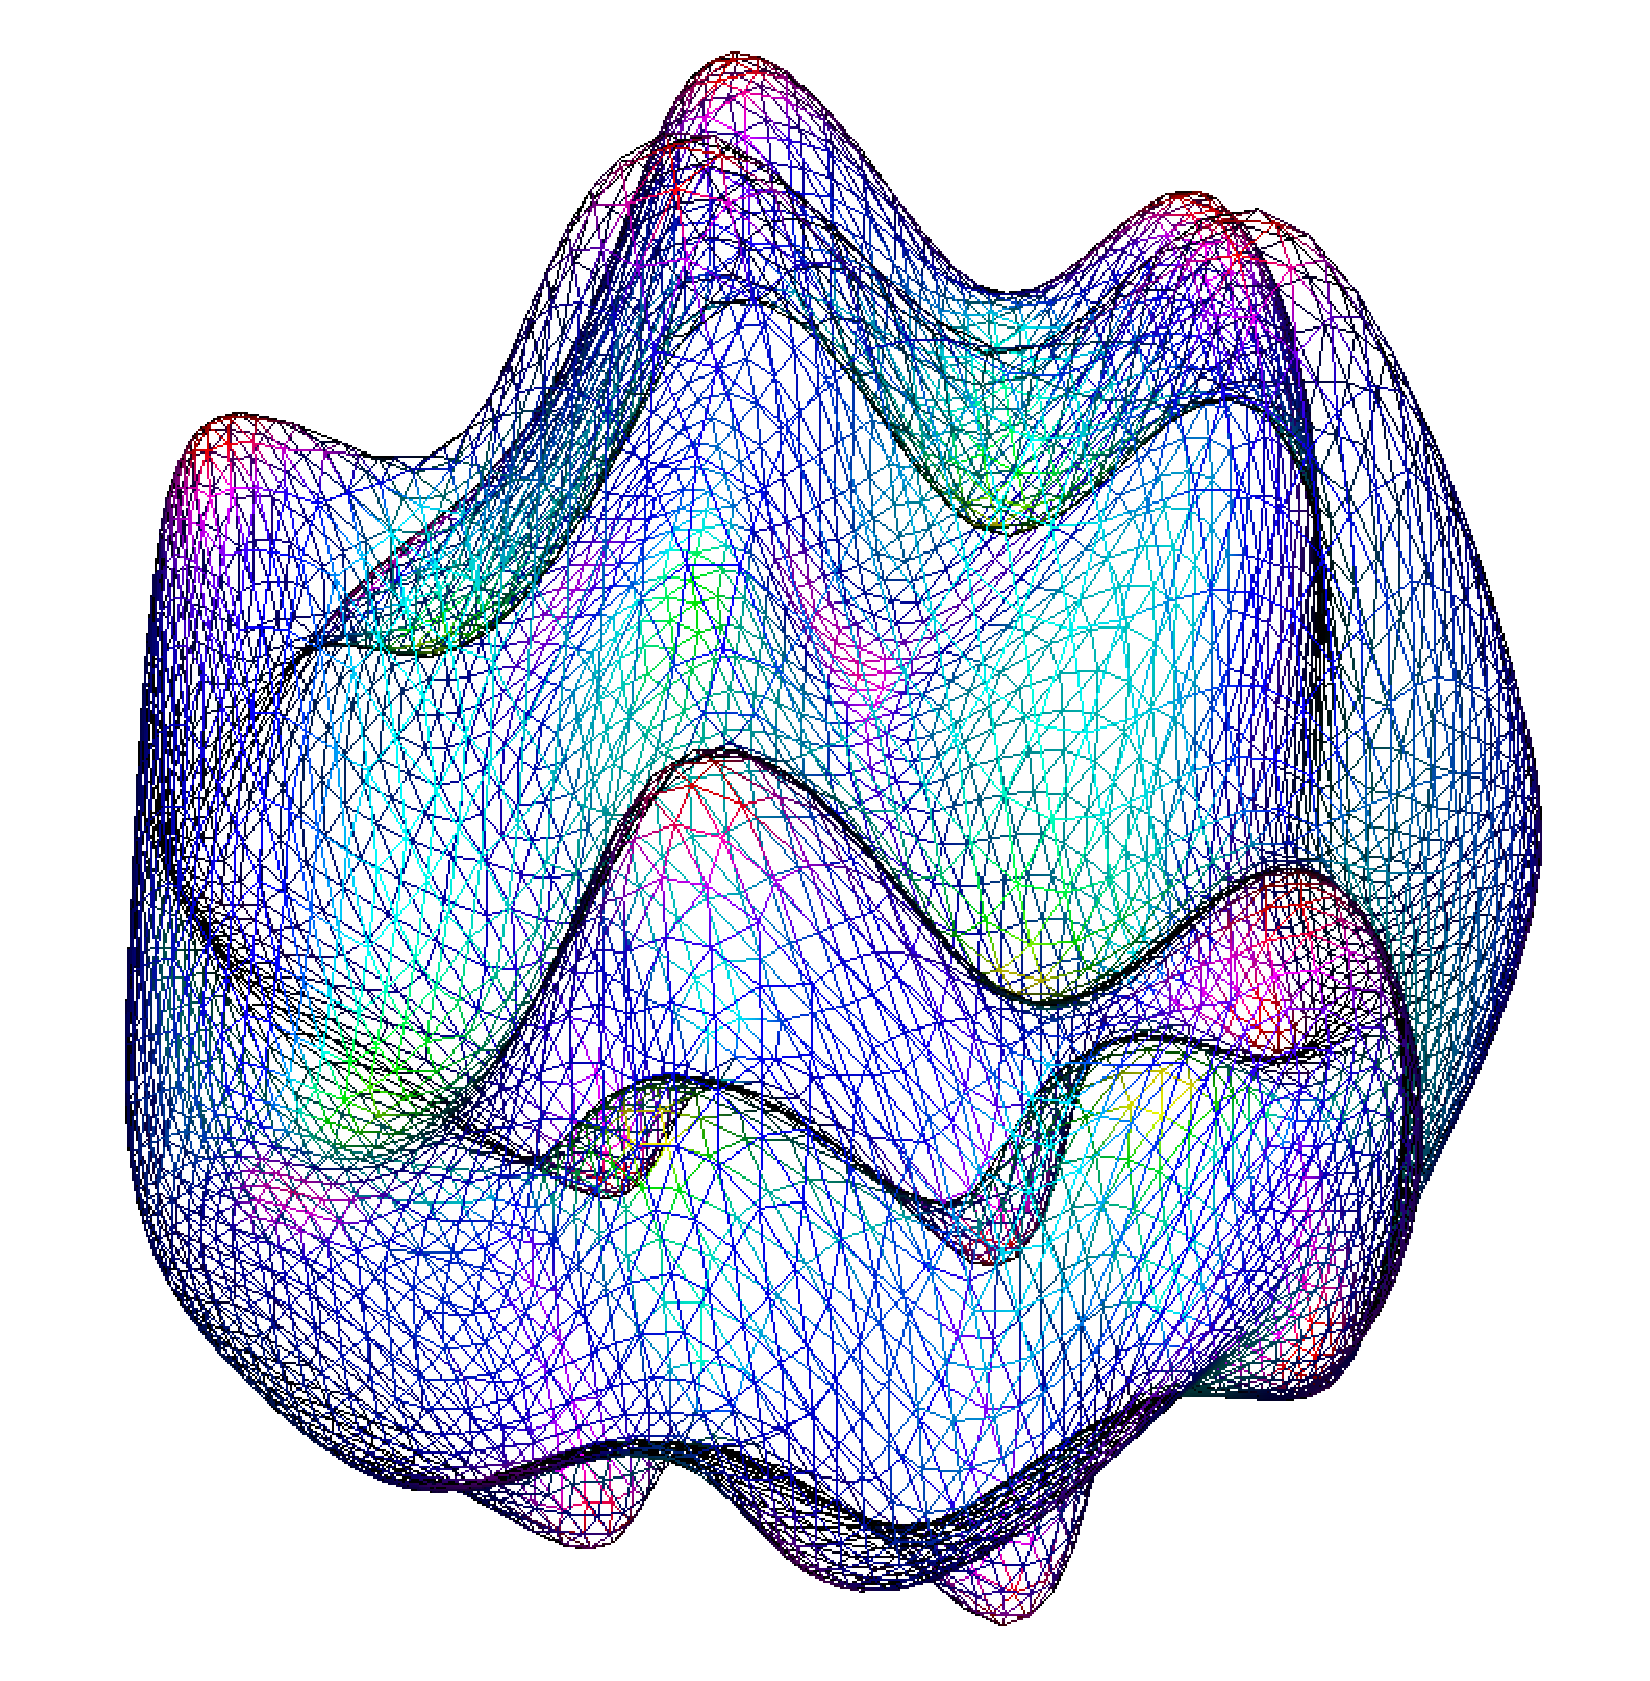
\includegraphics[width=5cm]{nice-mesh.eps} \label{fig:nice-mesh}}
    \end{center}
    \vspace{-.25in} \caption{The Original Data} \label{fig:original}
  \end{figure}  

  In Figure~\ref{fig:results}, we show the conformally flattened
  result of the filter. The coloring provides a convenient visual
  mapping from the original mesh to the sphere. In
  Figure~\ref{fig:nice-flat}, we show the surface view of the sphere
  and in Figure~\ref{fig:nice-flat-mesh}, we show the triangulated
  mesh on the sphere.

  \begin{figure}[h]
		\begin{center}
			\subfigure[Flattened Surface]{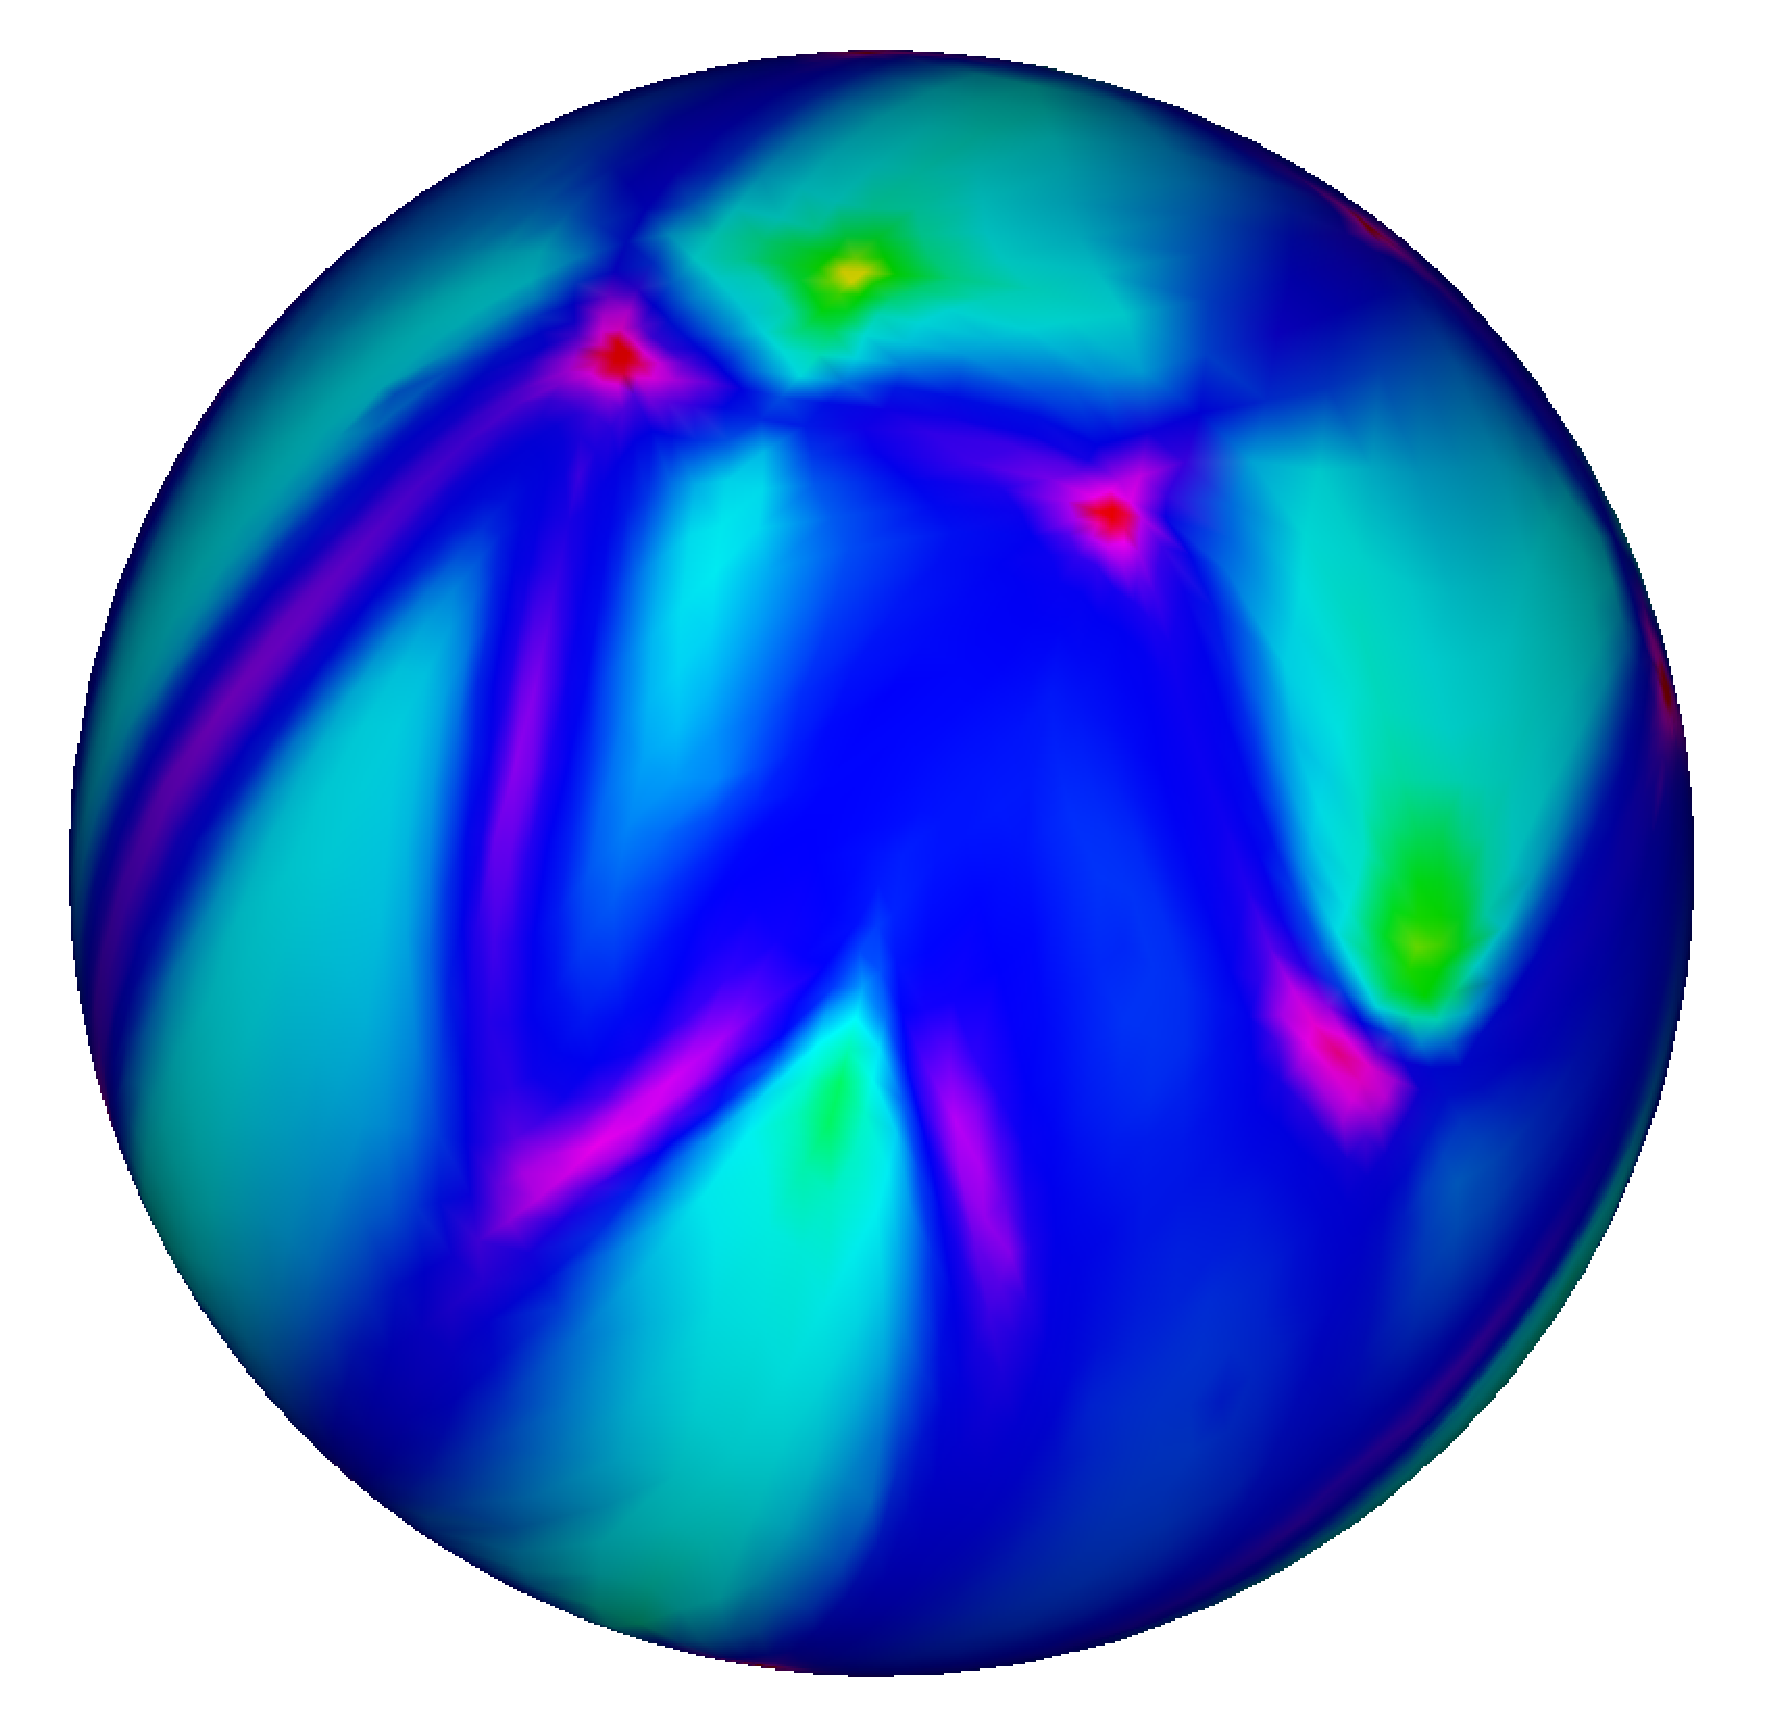
\includegraphics[width=5cm]{nice-flat.eps} \label{fig:nice-flat}}
			\subfigure[Flattened Mesh]{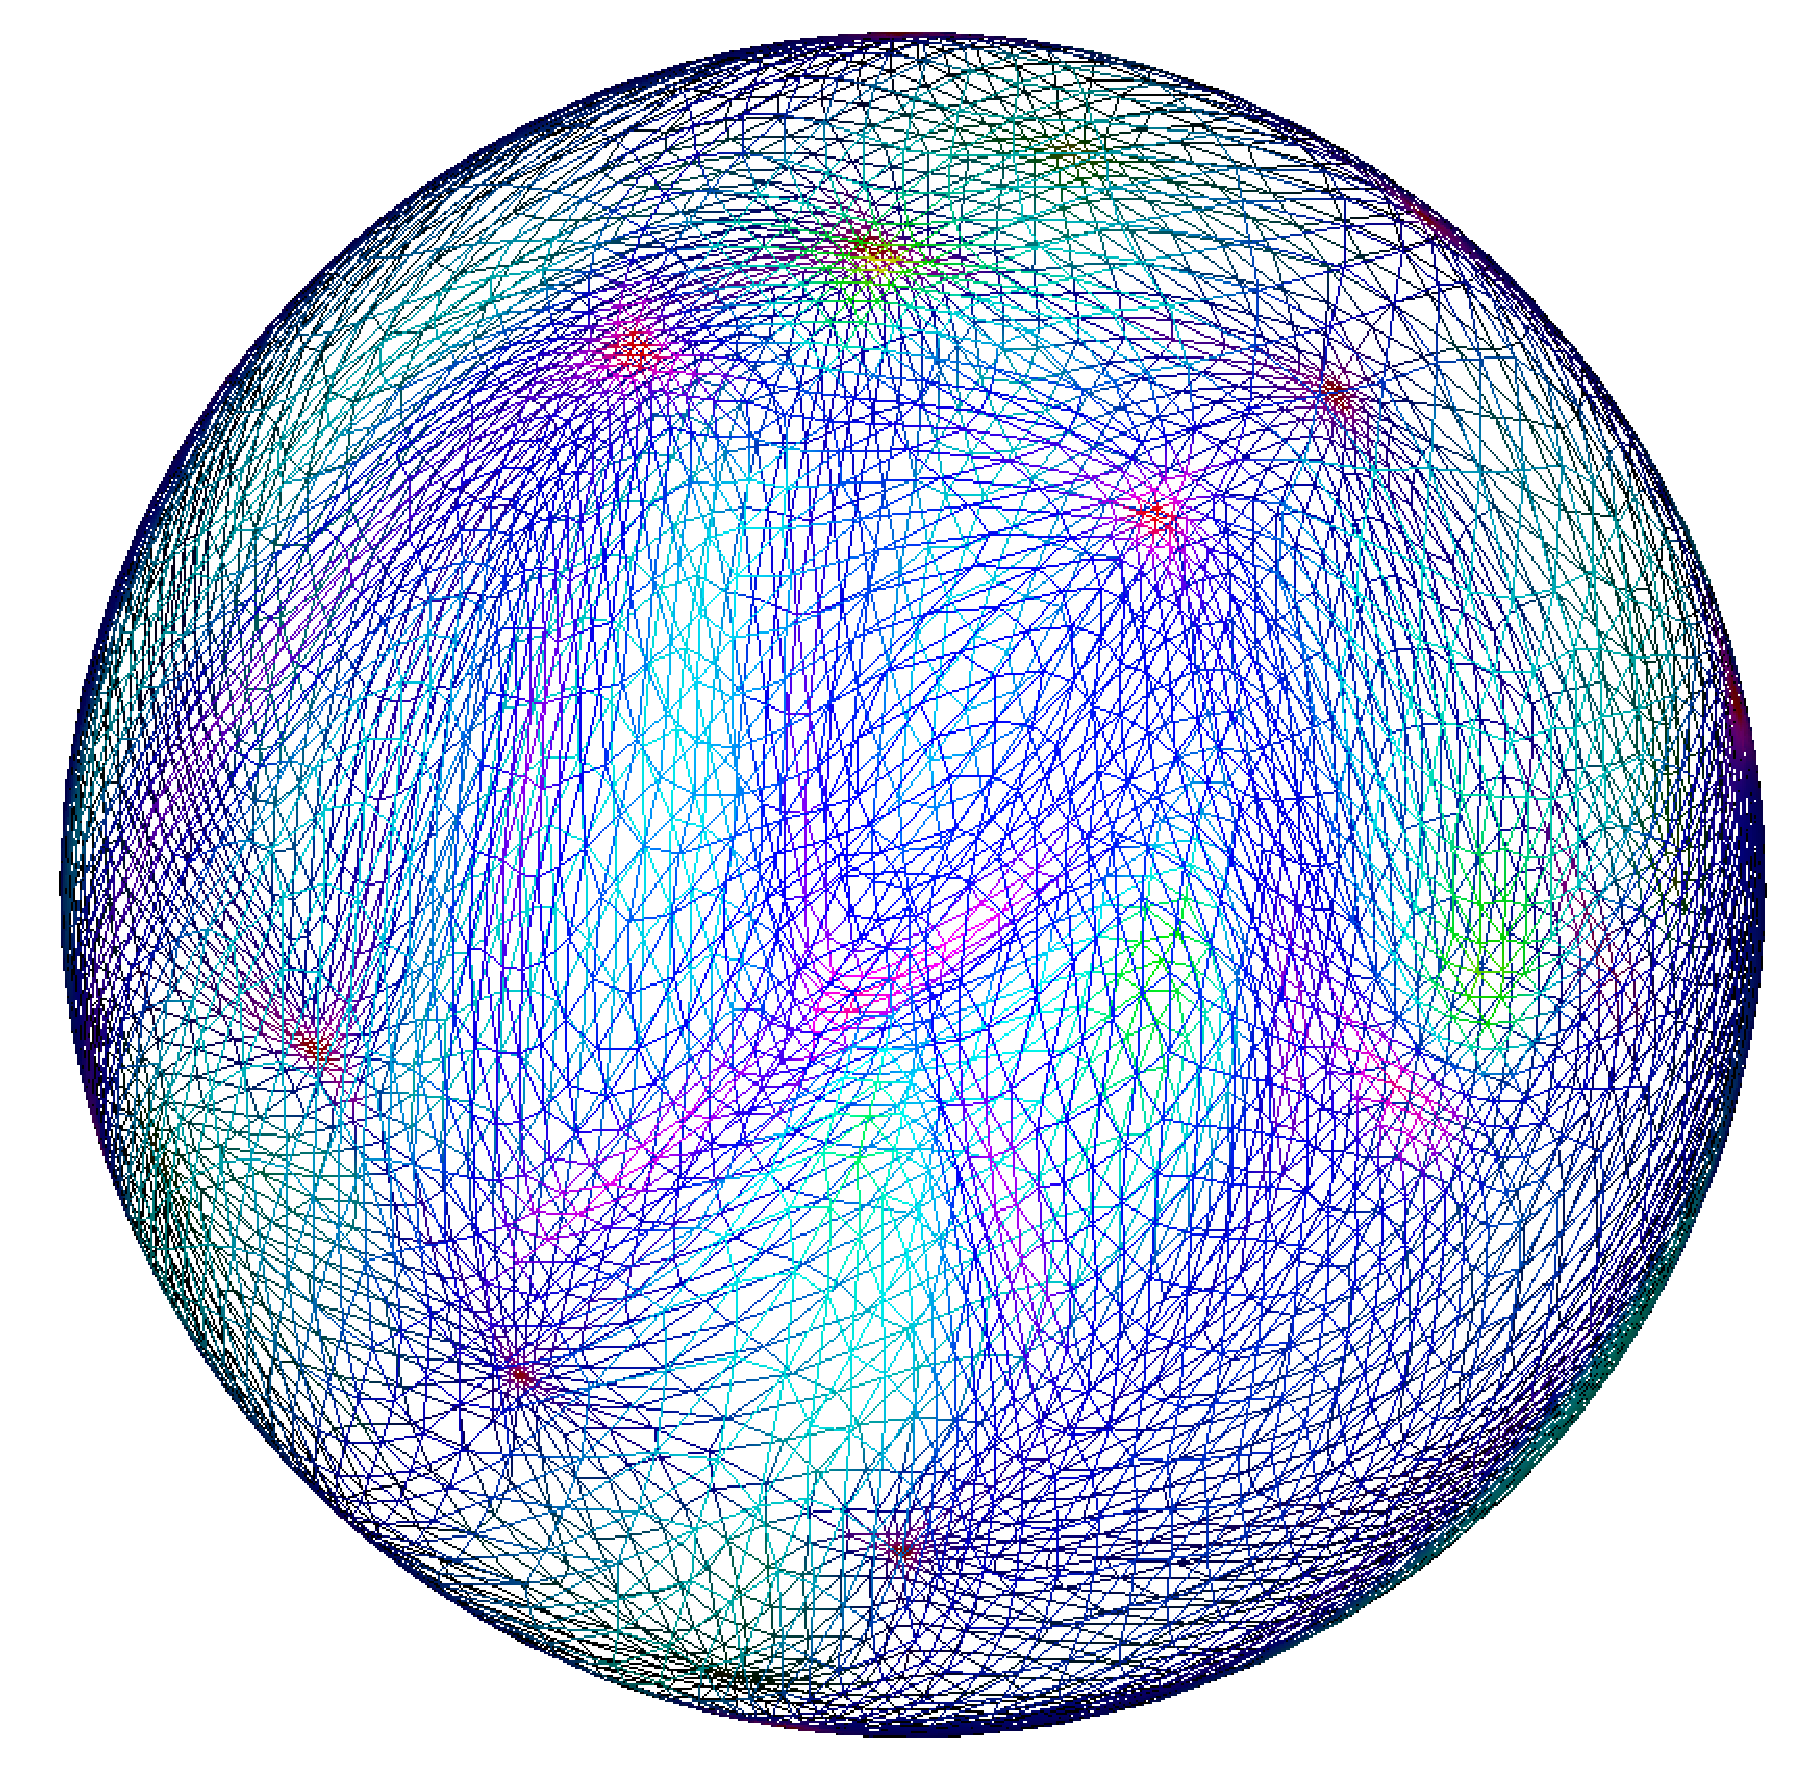
\includegraphics[width=5cm]{nice-flat-mesh.eps} \label{fig:nice-flat-mesh}}
    \end{center}
    \vspace{-.25in} \caption{The Results} \label{fig:results}
  \end{figure}  

  In order to reproduce our results, the reader should compile and run
  our code with the following packages (though the code will likely
  compile and run with other variants, including CVS checkouts, of
  CMake, ITK, and VTK):

  \begin{verbatim}
  CMake 2.2.3
  ITK 2.4.1
  VTK 4.4.2
  \end{verbatim}

  \noindent Note that this code is optimized for this particular
  $nice.vtk$ file and is not intended to be used with any generic
  mesh. There are two unique optimizations in this case:

  \begin{enumerate}
  \item The choice of the filter's scale parameter (using the setScale
  function. In this case, we chose: scale = 100.
  \item The choice of rendering options to fit the scale of the mean
  curvature values (see our Display function in the
  itkConformalFlatteningFilterTest.cxx file).
  \end{enumerate}

  \noindent In the next section, we show code that is
  optimized for a brain surface dataset.

  We have also included the results presented here as the
  $niceFlat.vtk$ file included in this submission. One can verify the
  angle preserving nature of this filter by comparing the relative
  angle proportions of angles emanating from each vertex in the
  mesh. We have included the anglePreserveCheck.cxx/h files to
  enable the user to verify that the angles are indeed preserved. We
  expond more on this in the next section.

	\section{Brain Flattening Applications}
  \label{sec:brain-flat}
  We propose to use this filter to conformally flatten brain
  surfaces. In order to accomplish this, we are currently
  investigating automated methods for extracting genus zero brain
  surfaces from raw MRI volumes.

  We have tried a variety of brain extraction (skull-removing) tools,
  including FreeSurfer, BET, MRIcro, ITKSNAP, and other ITK levelset
  filters and have been able to extract brain surface meshes using
  these tools. However, thus far, we have been unsuccessful in
  obtaining a \emph{genus zero} surface without significant manual
  editing, using these tools. We are hopeful that topology preserving
  levelset algorithms will soon become part of ITK to facilitate our
  work. The development of this filter is beyond the scope of this
  paper. We are also aware of topology correction algorithms which
  perform cutting operations to convert any particular genus surface
  into a genus zero surface. We will also investigate the use of these
  algorithms to extract genus zero brain surfaces.

  \begin{figure}[t]
		\begin{center}
			\subfigure[Original Brain Surface]{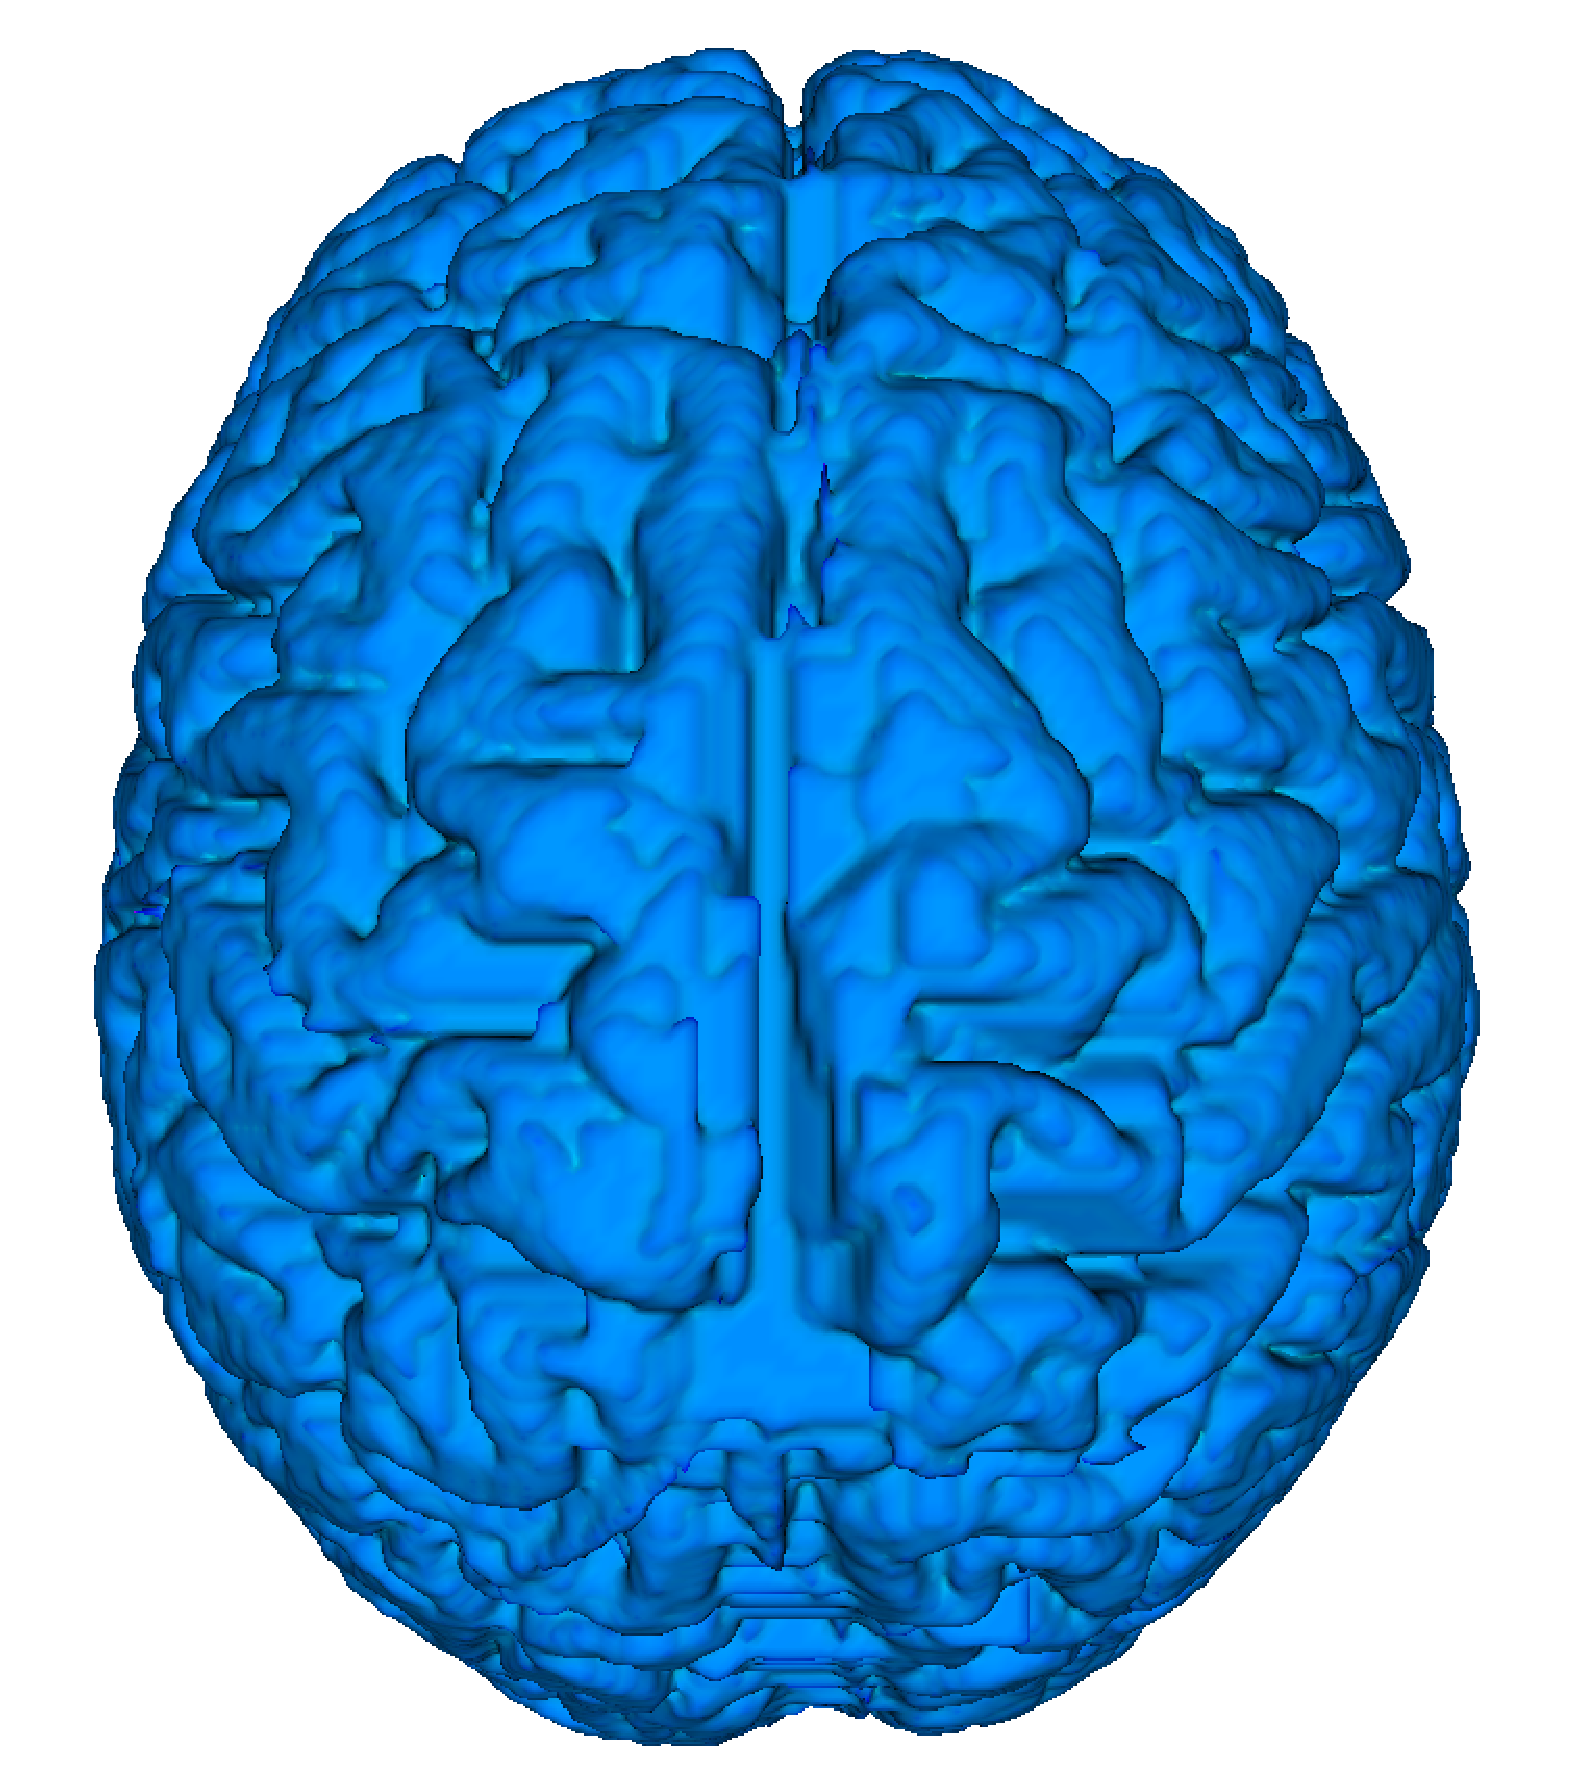
\includegraphics[width=5cm]{brain.eps} \label{fig:brain}}
			\subfigure[Original Brain Mesh]{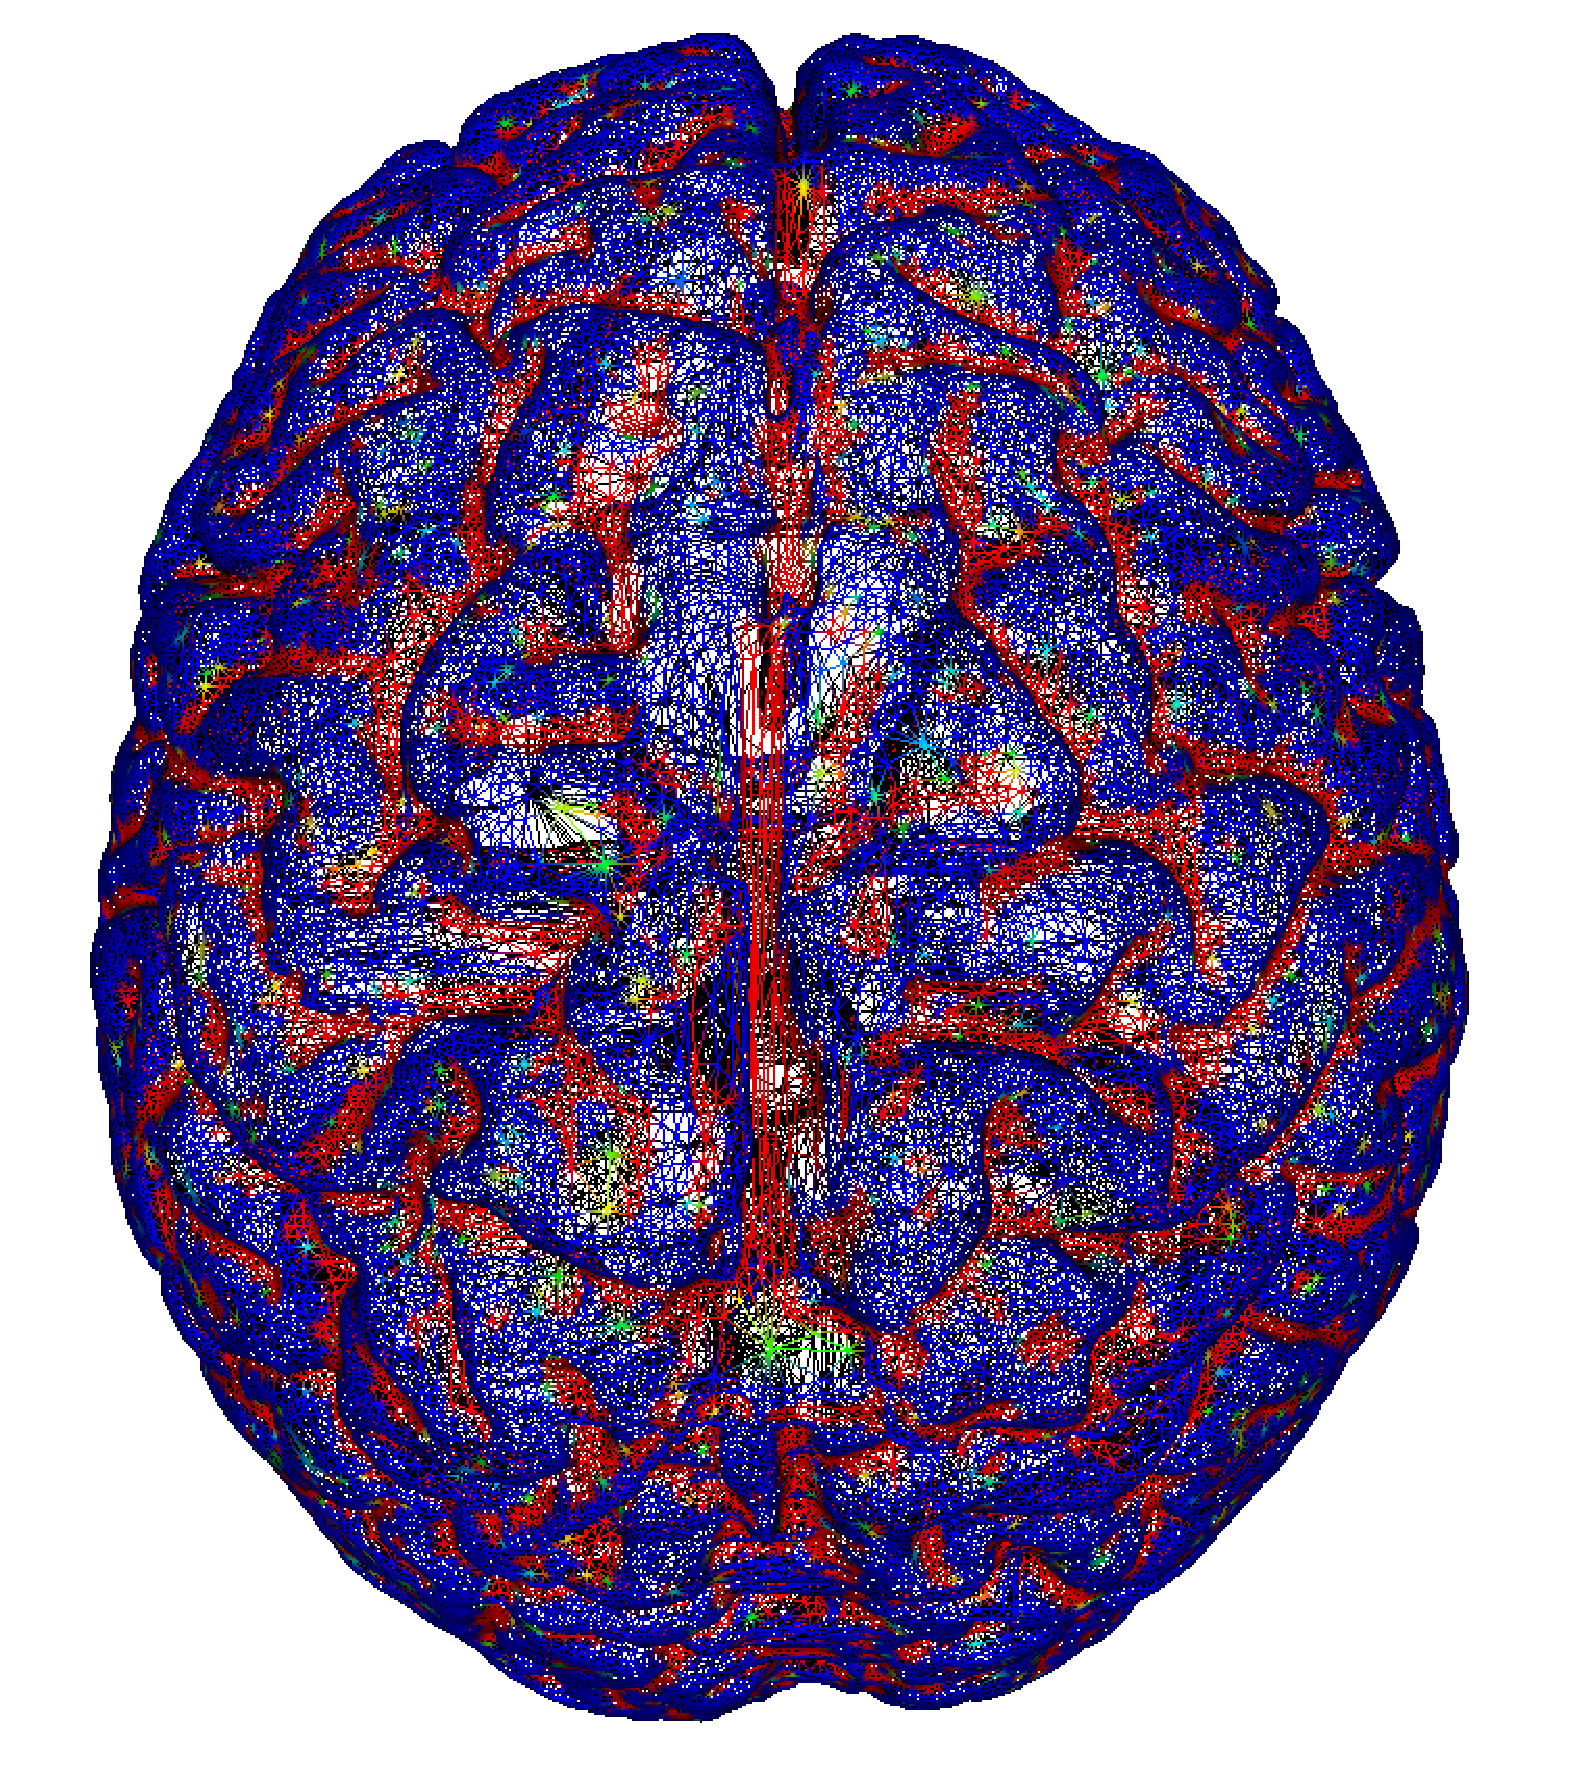
\includegraphics[width=5cm]{brain-mesh.eps} \label{fig:brain-mesh}}
    \end{center}
    \vspace{-.25in} \caption{Original Brain Surface}
  \end{figure}  

  As described above, through the use of various open-source tools and
  a fair amount of manual editing, we were able to obtain a genus zero
  surface of the brain which we show in Figures~\ref{fig:brain}
  and~\ref{fig:brain-mesh}. The result of running the brainTest.cxx on
  $brain.vtk$ can be seen in Figures~\ref{fig:brain-flat}
  and~\ref{fig:brain-flat-mesh}. We include the output file in this
  submission as $brainFlat.vtk$.

  \begin{figure}[h]
		\begin{center}
			\subfigure[Flattened Brain Surface]{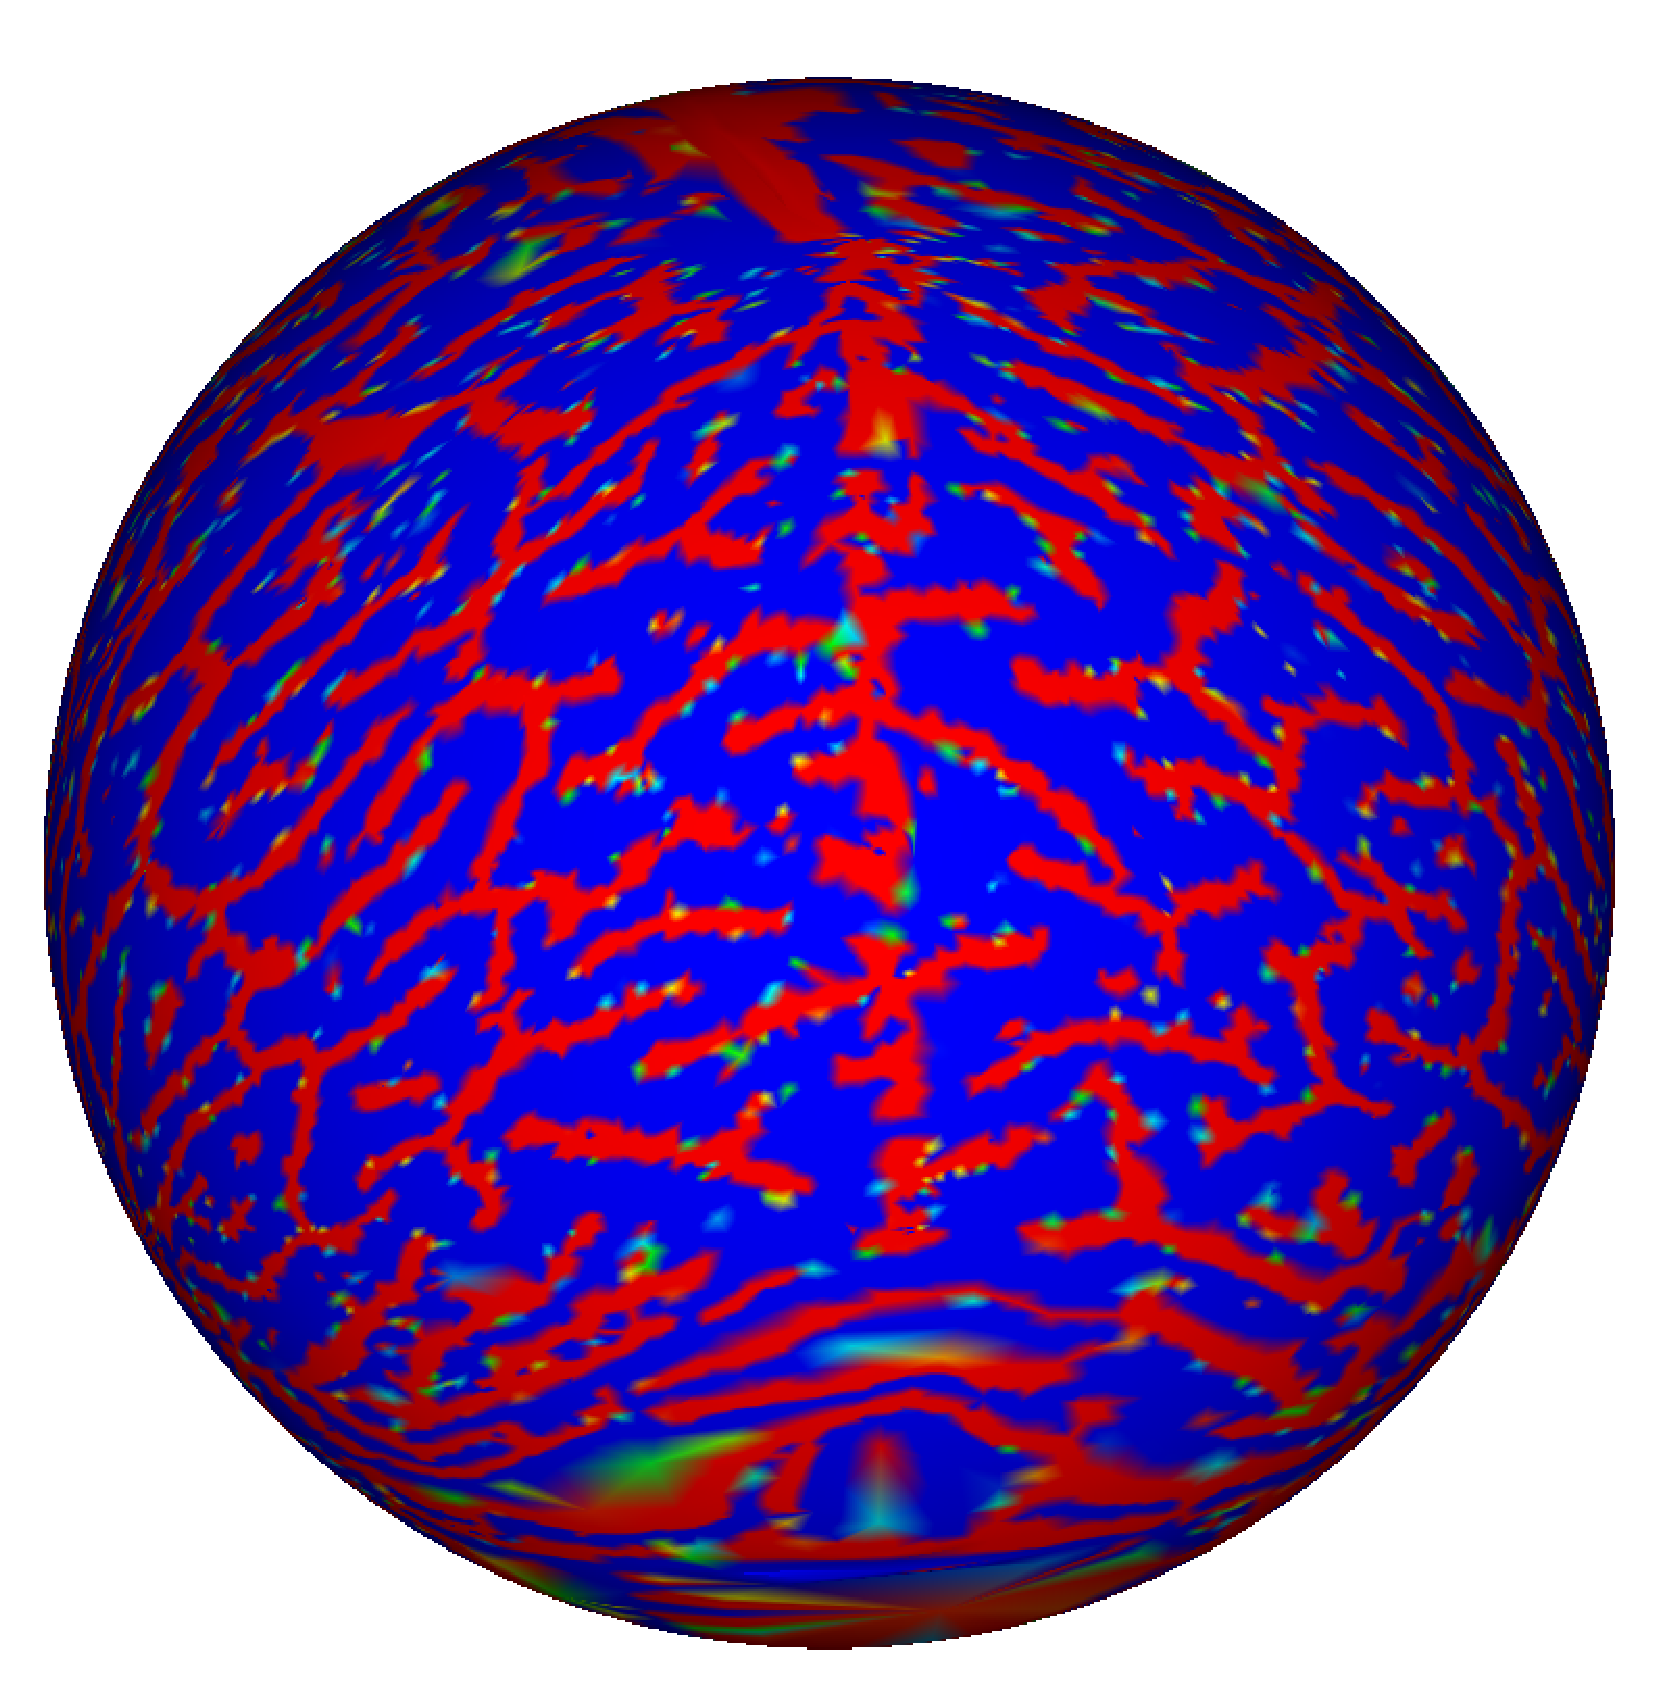
\includegraphics[width=5cm]{brain-flat.eps} \label{fig:brain-flat}}
			\subfigure[Flattened Brain Mesh]{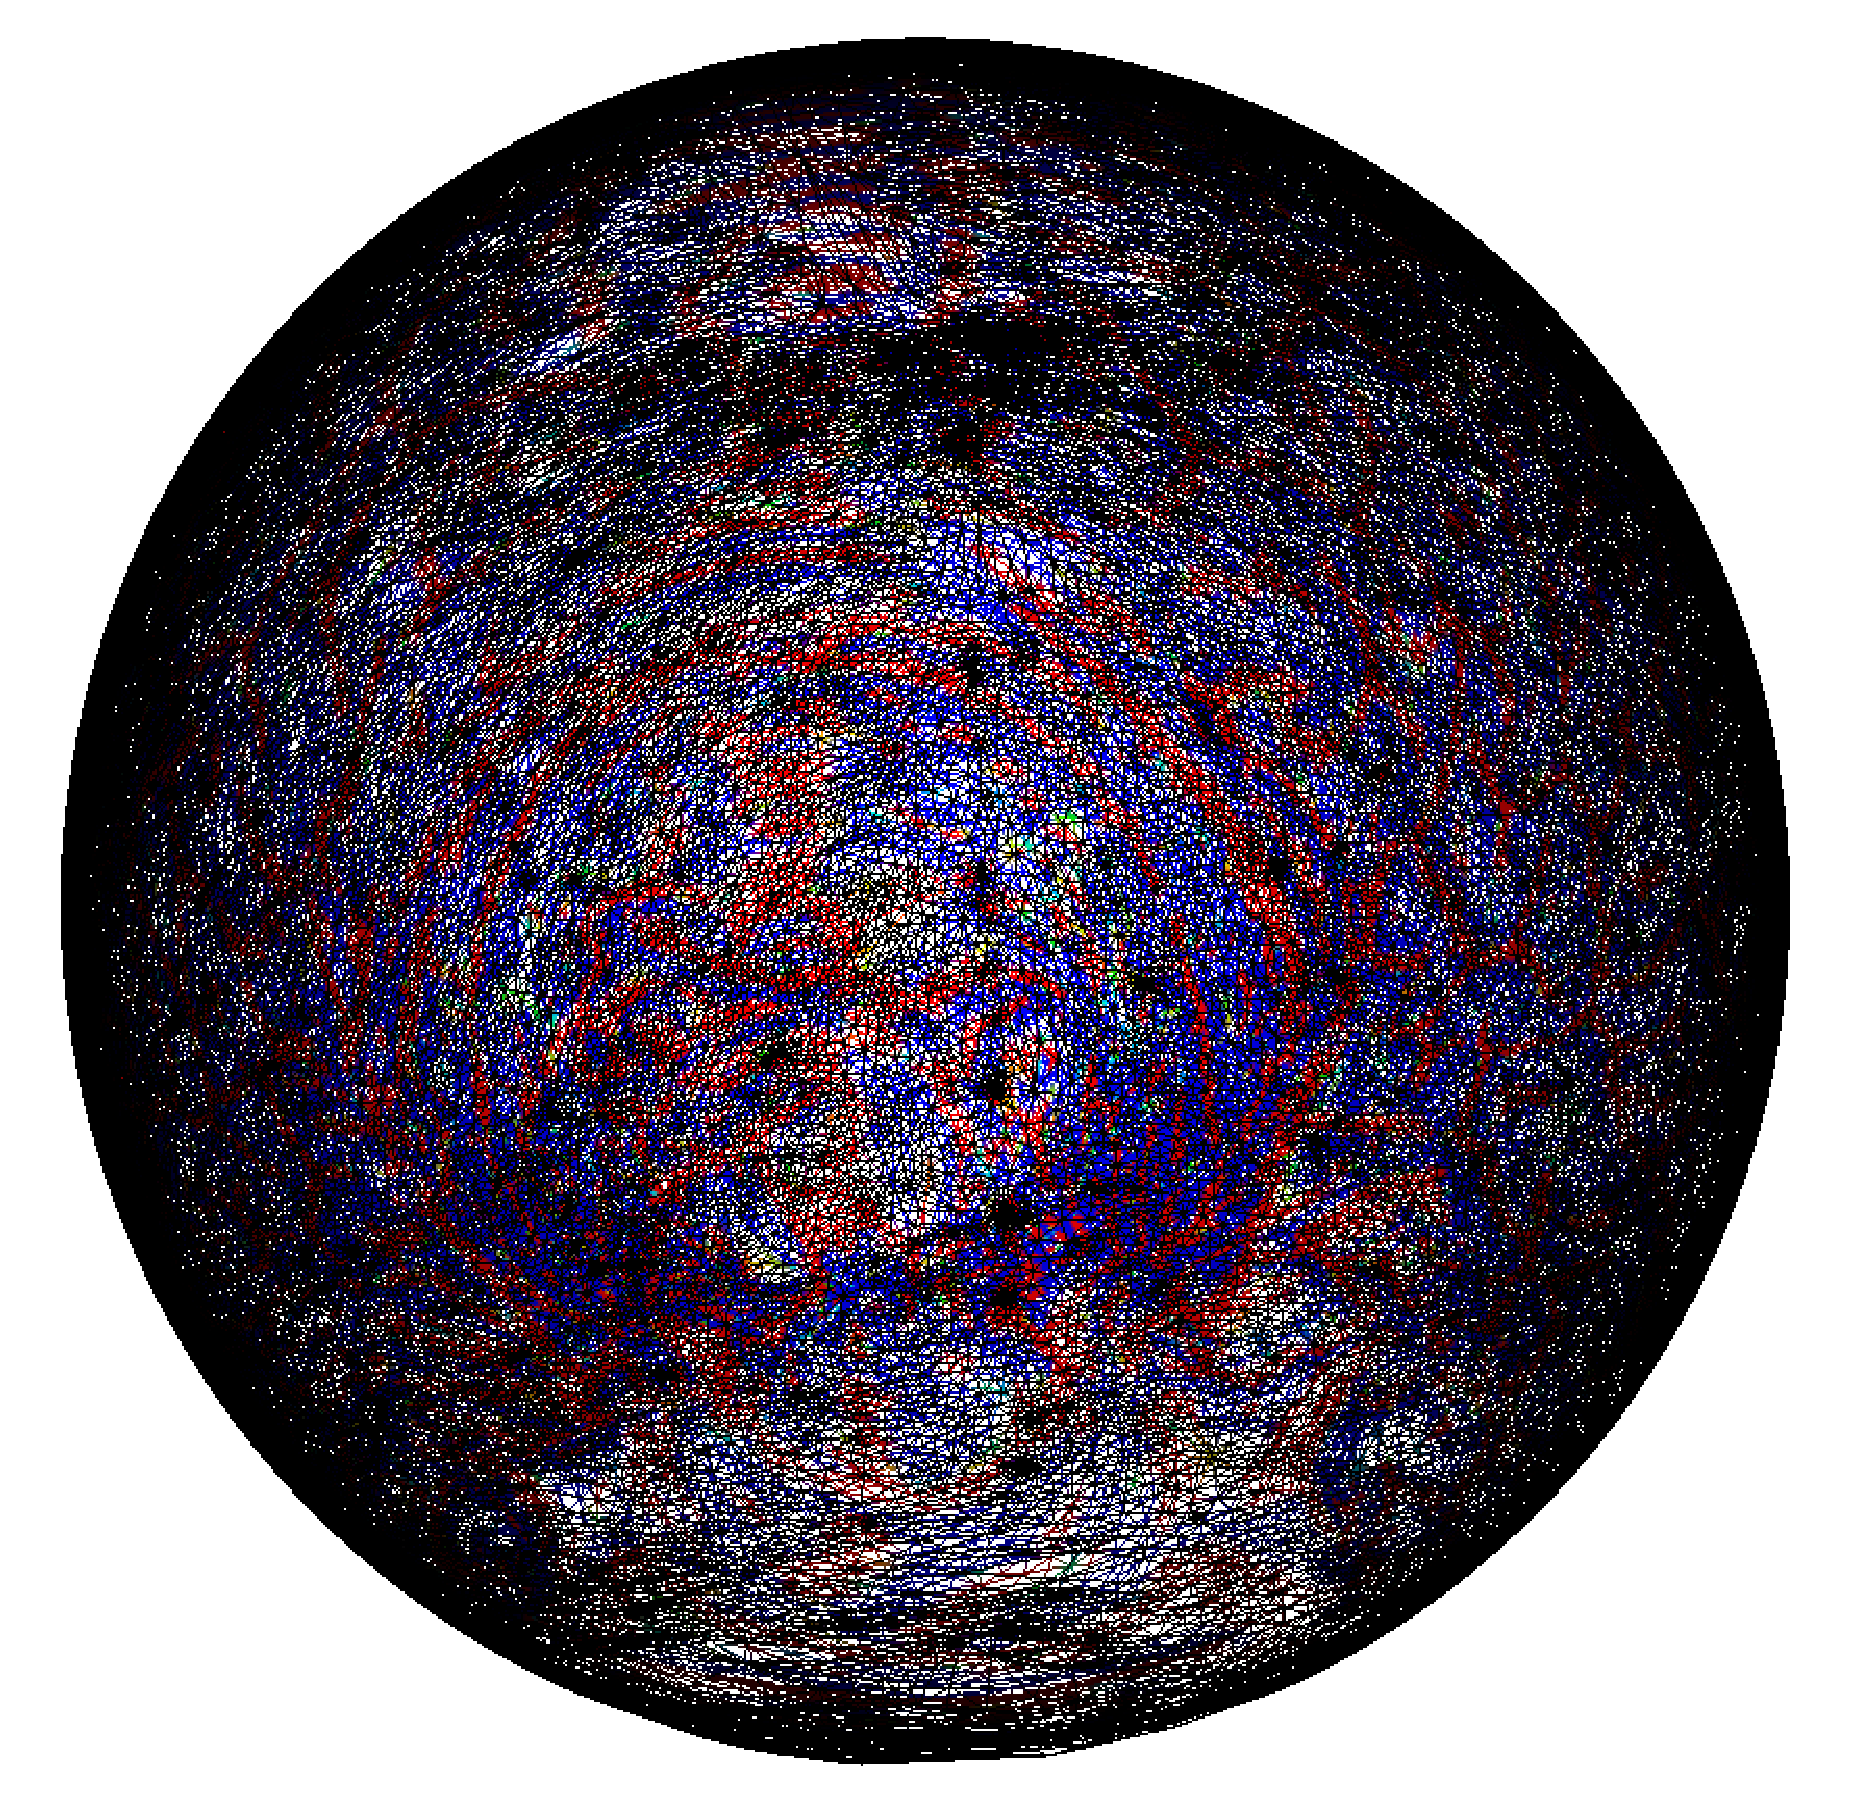
\includegraphics[width=5cm]{brain-flat-mesh.eps} \label{fig:brain-flat-mesh}}
    \end{center}
    \vspace{-.25in} \caption{Flattened Brain Surface}
  \end{figure}  

  We made the following optimizations in brainTest.cxx to achieve
  these results:

  \begin{enumerate}
  \item The choice of the filter's scale parameter (using the setScale
  function. In this case, we chose: scale = 5000.
  \item The choice of rendering options to fit the scale of the mean
  curvature values (see our Display function in the brainTest.cxx
  file).
  \end{enumerate}
  
  The mapping is conformal thus preserves angles. Since the surface is
  triangulated, the angle preserving property preserves the relative
  angles emanating from any given vertex in the mesh. Take, for
  example, any vertex $P$, which is mapped to point $P'$. There are
  $M$ angles emanating from $P$, denoted as $A_1, A_2, \hdots ,A_M$
  for the original mesh and $A'_1, A'_2, \hdots ,A'_M$ for the
  flattened mesh. The angle preserving property claims that
  \begin{eqnarray}
    \frac{A_k}{sum_{i=1}^M A_i} = \frac{A'_k}{sum_{i=1}^M A'_i}, \quad \forall k
    \label{anglePreserve}
  \end{eqnarray} 
  
  Numerically, the ratio of the left to right sides of equation
  (\ref{anglePreserve}) will be close to 1.0. We provide code to
  calculate and write to file the ratio in equation
  (\ref{anglePreserve}) for every angle at every vertex in the
  mesh. The usage of this angle preserving check is:
  \begin{verbatim}
  > ./anglePreserveCheck originalSurface.vtk flattenedSurface.vtk
  \end{verbatim}
  \noindent The computed ratios will be written to
  $angleRatioDiff.dat$. 

  For the example given in Figure~\ref{fig:nice}, the mean of all the
  ratios is 1.0026 and the standard deviation is 0.0629, thus
  verifying the angle preserving nature of this mapping.
  
	\section{Conclusions}
	In this paper, we have described the Insight Toolkit (ITK) Conformal
	Flattening filter: itkConformalFlatteningFilter. This ITK filter is
	an implementation of a paper by Sigurd Angenent, et al., ``On the
	Laplace-Beltrami Operator and Brain Surface Flattening''
	\cite{angenent1999lbo}. This filter performs an angle preserving map
	of any genus zero (i.e. no handles) triangulated mesh to the sphere
	or, alternatively, to the plane.

	We have provide the user with details to be able to reproduce our
	results. We have also given suggestions as to how to exploit the
	full functionality of this filter.

	Perhaps clinical studies of the resulting flattened map with yield
	insights into brain anatomy and function.



	% The preceding sections will have been written in a gentler,
	% introductory style.  You may also wish to include a reference
	% section, documenting all the functions/exceptions/constants.
	% Often, these will be placed in separate files and input like this:



	%\appendix
	%
	%\section{This is an Appendix}
	%
	%To create an appendix in a Insight HOWTO document, use markup like
	%this:
	%
	%\begin{verbatim}
	%\appendix
	%
	%\section{This is an Appendix}
	%
	%To create an appendix in a Insight HOWTO document, ....
	%
	%
	%\section{This is another}
	%
	%Just add another \section{}, but don't say \appendix again.
	%\end{verbatim}


	%%%%%%%%%%%%%%%%%%%%%%%%%%%%%%%%%%%%%%%%%%%%%%%%%%%%%%%%%%
	%
	%  Example on how to insert a figure
	%
	%%%%%%%%%%%%%%%%%%%%%%%%%%%%%%%%%%%%%%%%%%%%%%%%%%%%%%%%%%

	%\begin{figure}
	%\center
	%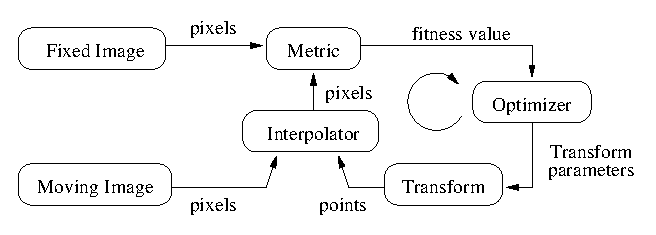
\includegraphics[width=0.8\textwidth]{RegistrationComponentsDiagram.eps}
	%\itkcaption[Registration Framework Components]{The basic components of the
	%registration framework are two input images, a transform, a metric, an
	%interpolator and an optimizer.}
	%\label{fig:RegistrationComponents}
	%\end{figure}



	%%%%%%%%%%%%%%%%%%%%%%%%%%%%%%%%%%%%%%%%%%%%%%%%%%%%%%%%%%
	%
	%  Example on how to insert an equation.
	%  Never forget to put an equation in your paper.
	%  They make them look professional and impress the reviewers.
	%
	%%%%%%%%%%%%%%%%%%%%%%%%%%%%%%%%%%%%%%%%%%%%%%%%%%%%%%%%%%


	%To support shape-guidance, the generic level set equation
	%(Eqn(~\ref{eqn:ShapeInfluenceTerm})) is extended to incorporate a shape guidance
	%term:
	%
	%\begin{equation}
	%\label{eqn:ShapeInfluenceTerm}
	%\xi \left(\psi^{*}(\mathbf{x}) - \psi(\mathbf{x})\right)
	%\end{equation}




	%%%%%%%%%%%%%%%%%%%%%%%%%%%%%%%%%%%%%%%%%
	%
	%  Insert the bibliography using BibTeX
	%
	%%%%%%%%%%%%%%%%%%%%%%%%%%%%%%%%%%%%%%%%%

	\bibliographystyle{plain}
	\bibliography{itkConformalFlattening06-IJ}


\end{document}
